\chapter{Cloud-SAP}

\chapterintro{ This chapter introduces the reference architecture known as Cloud-SAP, highlights its core concepts and indicates possible implementation ideas.
}

\section{Motivation}
As one can see, latest advances in providing platform-as-a-service still do not yield a comprehensive solution that embraces a range of fine-grained actions relevant to a given situation in an environment, as it was summarised in previous chapter. All of the presented solutions solely engage horizontal scaling, while other IT processes and corresponding actions such as vertical scaling, cloud bursting or application platform restart remains neglected. What is more, none of the investigated systems is a self-managing one, taking passive approach in enforcing given QoS. To make matter worse, some platforms such as Carina or OneFlow are provider-specific, hence, requiring vast knowledge and time of entities responsible for its supervision.

What system has all of the above-mentioned features is an autonomic one \cite{IBM06}, characterised by a self-management ability and driven by four crucial attributes:
\begin{itemize}
 \item \emph{self-configuration} - dynamic adaptation to changing environment such as provisioning new application instances, application tuning, traffic delegation to an external provider
  \item \emph{self-healing} - discovering, diagnosing and reacting to environment disruption such as container outage
  \item \emph{self-optimising} - monitoring and tuning resources: migrating containers, offloading traffic, for example
  \item \emph{self-protecting} - detecting and protecting against threats such as Deny-of-Service by provisioning extra resources
\end{itemize}

Beside this, key customer values such as IT process execution cost or time needed to complete it are enhanced through rapid process initiation and reduced time and skill requirements \cite{IBM06}. As specified in blueprint, applying autonomic system to manage application environment is possible because following conditions are met:

These four system capabilities combined together yield a promising architecture from QoS ensuring perspective. Beside this, key customer values such as IT process execution cost or time needed to complete it are enhanced through rapid process initiation and reduced time and skill requirements \cite{IBM06}. As specified in blueprint, applying autonomic system to manage application environment is possible because following conditions are met:
\begin{itemize}
  \item tasks involved in associated IT process needs to be automated
  \item it is possible to initiate processes based on observable and detectable situations
  \item autonomic manager posses sufficient knowledge
\end{itemize}

Cloud Self Adaptive Platform (Cloud-SAP) is a reference architecture aspiring to supply application providers with an autonomic computing environment. Figure \ref{img:architecture-context} shows Cloud-SAP place in an exemplary application provisioning request. 
\begin{figure}[!ht]
  \begin{center}
    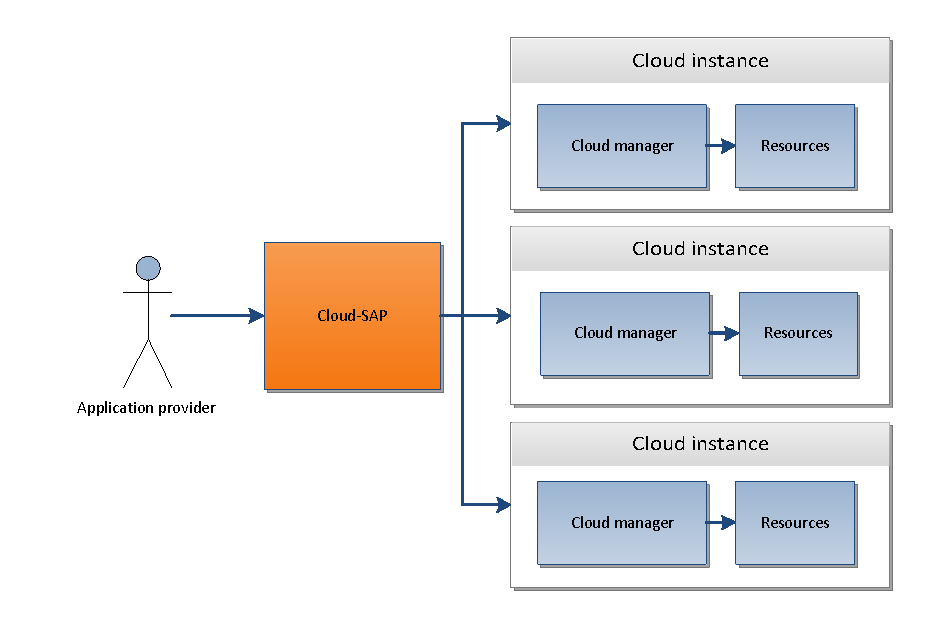
\includegraphics[width=0.9\textwidth]{chapter-design/architecture-context}
  \end{center}
  \caption{Cloud-SAP place in an exemplary application provisioning request}
  \label{img:architecture-context}
\end{figure}

Application providers can be both end-users or other system interfaces, Cloud-SAP is suitable for both cases. Cloud-SAP is entirely cloud providers and resources agnostic as long as they externalise management interfaces.

Successive sections define core layers of a Cloud-SAP and give insight into possible implementation decisions, while the next chapter presents a proof-of-concept implementation.

\section{Overview}
The previous section dealt with all premises that led to a conclusion that the proposed architecture can rely heavily on the concept of an autonomic system. In this section the further elaboration on the solution is presented.
Figure \ref{img:architecture-context} showed the context which the architecture applies to. As one can see, Cloud-SAP can be seen as a proxy between the user and cloud instances and as a coordinator of the latter. Although cloud instance itself consists of a cloud manager and additional resources, in general, it is perfectly legitimate to consider it a resource as well. 

Before the more detailed diagram of the solution is presented, it is essential to introduce another indispensable function that lies in the heart of any autonomic entity -- its ability to detect an undesirable state and take appropriate actions. This is achieved by the presence of a \emph{control loop} which collects data about the environment, analyzes it and takes all needed steps to recover the system. Not only can the attributes introduced in the previous section be bound to an autonomic system, but they can also be thought of main and broad categories of a control loop \cite{IBM06}.

Having said so, we are ready to give a layered overview of a proposed solution, which is shown in figure \ref{img:csap-layered-structure}.
\begin{figure}[!ht]
  \begin{center}
    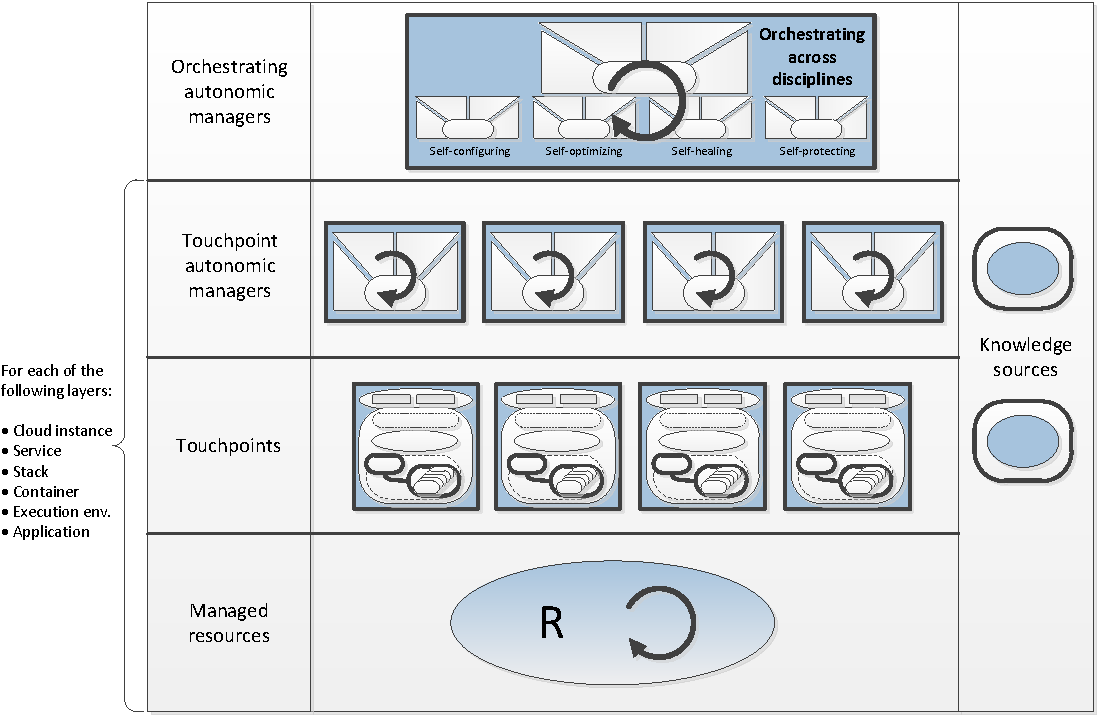
\includegraphics[width=\textwidth]{chapter-design/csap-layers}
  \end{center}
  \caption{Cloud-SAP components}
  \label{img:csap-layered-structure}
\end{figure}

The building blocks of the architecture are:
\begin{itemize}
  \item Managed resources
  \item Touchpoints
  \item Touchpoint autonomic managers
  \item Orchestrating autonomic managers
  \item Knowledge source
\end{itemize}
As resources were identified on various levels of abstraction, starting from the application that is to be deployed and ending on a cloud instance that aggregates different applications and services, we can think of the last three layers (managed resources, touchpoints and touchpoint autonomic managers) as a one logical component which can aggregate and manage other components. This recursive definition applies to identified managed resources described in the next section, apart from application as we consider it the most fundamental and indivisible resource.

\subsection{Managed resources}
\emph{Managed resources} form the lowest layer of a stack. When it comes to application provisioning in a cloud environment we can think of the following resources:
\begin{itemize}
  \item \emph{Application} -- application itself can be considered resources which can be managed by an external entity, e.g. by restarting/killing it,
  \item \emph{Execution environment of an application} forms an inherent part of an application lifecycle and its proper tuning can greatly influence its performance,
  \item \emph{Container} -- an isolated and controlled environment in which applications are deployed,
  \item \emph{Stack} -- every application has a technology stack associated with it; what is more, if we confine ourselves to map one instance of a container with only one application, we can think of stack as a composition of application (and its execution environment) and a container,
  \item \emph{Service} -- more complex solutions/applications require interactions with various components that are not necessarily implemented using the same technology stack; service denotes a logical entity that consists of a list of stacks that should form one, indivisible component,
  \item \emph{Cloud instance} -- an entity able to deploy \emph{services}
\end{itemize}
What is more, the listed resources are nested within one another and one's ability to work/run smoothly highly depends on the condition and state of the resource it forms part of. This is shown in figure \ref{img:managed-resources-aggregation}.
\begin{figure}[!ht]
  \begin{center}
    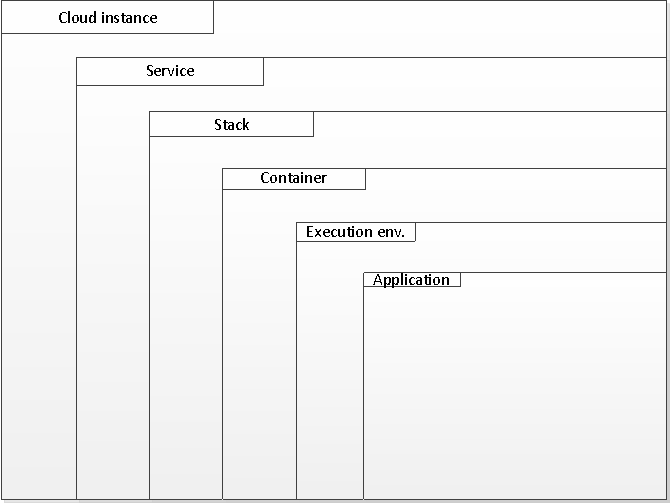
\includegraphics{chapter-design/csap-resources-aggregation}
  \end{center}
  \caption{\emph{Managed resources} identified by Cloud-SAP and their aggregation}
  \label{img:managed-resources-aggregation}
\end{figure}

As it is shown in figure \ref{img:csap-layered-structure}, each \emph{managed resource} can have embedded self-management control loop. The control loop may or may not be externally visible by the manageability interface. For example, an application can have \emph{self-configuring} control loop which performs appropriate runtime tuning of its configuration files, while not being visible (by not providing any API) and manageable by any entity.

\subsection{Touchpoints}
\emph{Touchpoint} forms the layer above managed resources. It has two main functions \cite{IBM06}:
\begin{inparaenum}[1)]
\item provides manageability interface and
\item implements \emph{sensor} and \emph{effector} behaviour.
\end{inparaenum}

By means of manageability interface, external entities can control managed resources. It can be done by, e.g. leveraging API, configuration files or logs. Additionally, it is possible to obtain information via touchpoint about the state of the resource. \emph{Sensor} and \emph{effector} behaviours refers to mechanisms that allows collecting data and change the behaviour of the resource, respectively.

\subsection{Touchpoint Autonomic Manager}
\emph{Touchpoint Autonomic Manager} is a component that implements the control loop behaviour and, in effect, manages the managed resources through exposed touchpoints. As it was stated in the previous sections, only four types of control loops are of an interest in the proposed architecture, i.e. \emph{self-configuring}, \emph{self-healing}, \emph{self-optimising} and \emph{self-protecting}.

The actions executed by each control loop on the assigned managed resource are defined in a \emph{policy} that is associated with the given autonomic manager. Thus, there is a one-to-one mapping between managed resource and touchpoint, and touchpoint and autonomic manager.

Each autonomic manager implements the control loop which can be split into four consecutive blocks, which share knowledge among one another. The output from one block forms an input to another. However, it is perfectly possible for a block to perform an action for its side effects, e.g. an action can result in producing relevant information contained in log files, which, in turn, comprises a piece of shared knowledge. Each block implements different behaviour based on the abstraction level and resource they operate on (see figure \ref{img:csap-layered-structure}). Nevertheless it is possible to define their generic behaviour, which embraces the following phases that correspond to a given block:
\begin{itemize}
  \item \emph{monitor} -- this function of autonomic manager is responsible for collecting and aggregating data about the resource it manages,
  \item \emph{analyse} -- this part takes the data from \emph{monitor} phase and perform in-depth analysis of it, which can result in, e.g. prediction plans. It is possible to incorporate more complex mechanisms, such as machine-learning, to fully use the obtained information for better prediction models,
  \item \emph{plan} -- this block is responsible for planning the appropriate action based on the output of the previous block and policies,
  \item \emph{execute} -- the goal of this function of autonomic manager is to execute the planned action
\end{itemize}
What is more, an autonomic manager exposes \emph{sensor} and \emph{effector} manageability interfaces which enables other entities (including other autonomic managers) to manage it in a similar manner as the component itself manages a resource. The image of an autonomic manager with its control loop and provided interface is shown in figure \ref{img:autonomic-component}.

\begin{figure}[!ht]
  \begin{center}
    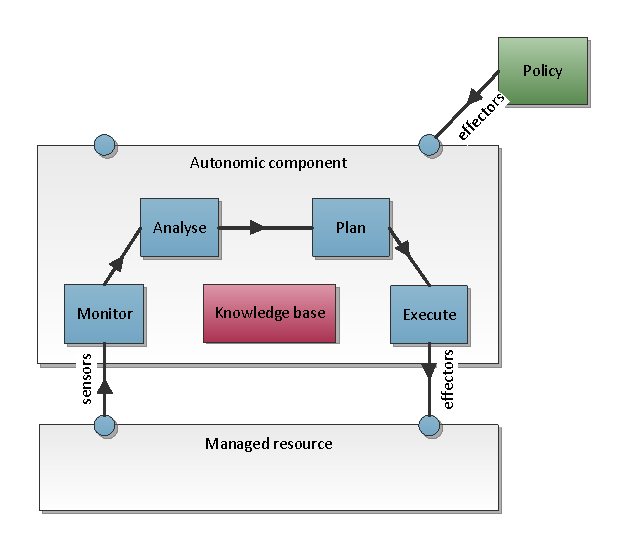
\includegraphics{chapter-design/autonomic-component}
  \end{center}
  \caption{Autonomic manager}
  \label{img:autonomic-component}
\end{figure}

\subsection{Orchestrating autonomic manager}
While an autonomic manager which manages a single resource may be satisfactory enough in many business cases, there are situations when additional coordination among managers is essential to attain the certain goal. This can result in incorporating autonomic behaviour within an entity in a system-wide scope.

Such a coordination can be achieved by introducing another autonomic manager whose sole purpose is to harmonize the work of dependent ones by extensive use of their \emph{sensor} and \emph{effector} interfaces. These managers are called \emph{orchestrating managers}.

When it comes to the complex task of ensuring the Quality of Service requirements for a client of a cloud computing environment, it is vital to ensure proper mechanisms that would allow seamless cooperation among different cloud providers. Such cooperation could result in a migration of an application between different clouds, market-driven choice of the cloud providers and so on.

As the exemplary actions can be regarded complex ones, they cannot be associated with actions taken by autonomic managers of only one type. Thus, an orchestrating autonomic manager should coordinate other managers of any type -- an arbitrary mixture of self-healing, self-configuring, self-optimizing and self-protecting managers. Employment of these concepts in Cloud-SAP will be discussed later in detail.

\subsection{Knowledge source}
\emph{Knowledge source} provides access to knowledge stored, for example, in a registry, dictionary or database. It is recommended that knowledge source share knowledge among multiple managers, consequently extending their capabilities by performing additional tasks covering recognising particular symptoms or applying specified policies, for instance.


Whilst knowledge can be expressed as symptoms, policies, change requests or history logs, Cloud-SAP differentiates its two main types:
\begin{itemize}
 \item \emph{policy} - set of constraints that, when evaluated, influence system behaviour and possibly trigger further actions. Cloud-SAP does not specify policy format, however, it is vital to employ only one format in whole system so it can be freely exchanged
 \item \emph{problem determination knowledge} - correlation of data, symptoms and decision trees determining actions that can be taken to eliminate symptoms
\end{itemize}

An autonomic manager can obtain knowledge in one of three ways:
\begin{itemize}
 \item \emph{receive it dynamically} - a common way for passing a policy to a manager. 
 \item \emph{retrieve it from external knowledge source} - an approach for obtaining symptom definitions or historical knowledge. For example, detailed history of a resource, its problems and actions taken can be retrieved from a log file.
 \item \emph{create it dynamically} - monitoring and execution phase are strictly correlated and consequently data received from sensors, actions taken by effectors and their result can be stored as a knowledge and provide valuable information during future problem investigations
\end{itemize}


\section{Autonomic application manager}

\section{Autonomic application platform manager}
%w kazdej sekcji opis MAPEK - co monitoruje, w jaki sposob analizuje i planuje, wykonuje

% darek
\section{Autonomic container manager}
It is expected that autonomic container manager supervise lifecycle of a container, modifying its properties accordingly to a given condition.

\subsection{Managed resource}
To recap, \emph{container} is an entity that provides an execution environment for an application platform. There is a variety of technologies that intend to provide an isolated, secure execution environment. Table \ref{tab:containeristation-technologies} groups them into three main categories: full virtualization, os-level virtualization, operating system process.

\begin{table}[!htbp]
  \centering
  \begin{tabularx}{\textwidth}[]{ X X X X }
    \specialrule{.1em}{.05em}{.05em} 
    & \textbf{Full virtualization} & \textbf{OS-level virtualization} & \textbf{OS process} \\
    \specialrule{.1em}{.05em}{.05em} 
    \textbf{Features} & 
-- complete simulation of machine's hardware

-- full isolation

-- host system is not shared among guests

    &
-- isolation is based on user-spaces

-- shared kernel

-- lesser overhead than full virutalization

-- effective i/o operations
    & 
-- custom solution that uses processes, cgroups, SELinux, for example

-- lesser overhead possible
    
\\ \hline
\textbf{Examples} &
-- KVM

-- Xen

-- VMware &

-- LXC

-- OpenVZ
&
-- OpenShift containers
\\ \hline
  \end{tabularx}
  \caption{Containerisation technologies}
  \label{tab:containeristation-technologies}
\end{table}

While choosing containerisation technique is entirely left to an implementation, Cloud-SAP recommends using os-level virtualization or operating system processes as they involve lesser resources and are more flexible, especially in terms of dynamic adjustment. Moreover, lightweight containers have been proved more effective than full virtualization in some scenarios: \cite{RaHiSj13}.

Not only can container be a managed resource but also it can have embedded control loop, depending on chosen mechanism. For example, Xen uses mechanism called 'memory ballooning' to intelligently distribute memory resources among guest systems what is in fact an example of self-optimising control loop. Though, embedded container loops are interesting they does not lie in Cloud-SAP area of interests and as a consequence are not further discussed.

Container uses variety of underlying resources such as storage or network connection. However, for simplicity, Cloud-SAP does not take them into consideration and therefore they are represented merely as a container properties not first-class resources.

\subsubsection{Touchpoint}
Container's touchpoint externalises hypervisor and operating system APIs. Similarly to all touchpoints, sensors for gathering data and effectors for influencing it can be distinguished. It is highly recommended for them to be linked, forming together manageability capabilities. In other words, property (i.e. CPU) can be read only when it is possible to set it as well. For instance, free / used CPU, free / used memory, network bandwidth, disk usage can be measured. Cloud-SAP requires free CPU to be at least supported.

\subsection{Autonomic controller}
\emph{Autonomic container controller} aims to automate container's management function and externalise its configuration through its interfaces. In order to do achieve that, it implements a control loop that fully covers container life cycle: gathering information about it, analysing it, planning and executing actions on top of that. These four functions along with knowledge necessary to perform them designate modular structure of a controller as shown in figure \ref{img:autonomic-component}.

\subsubsection{Monitoring}
As it was already mentioned, monitoring module aims to gather data from container's sensors. While Cloud-SAP does not have any specific requirements regarding underlying monitoring mechanism, there are a few aspects that should be taken into consideration:
\begin{asparaenum}
  \item[\textbf{Metrics}] rozne opcje: cpu, memory, co wybrac przynajmniej cpu

  \item[\textbf{Data filters}] co robic z danymi, agregowac, jesli tak to jak, trzeba niwelowac zaburzenia (art? o monitoringu)

  \item[\textbf{Persistence}] czy przechowywac dane, jesli tak to jakie, potrzebne do analizy, wyciagania wnioskow (dane, reakcja -> odpowiedz)

  \item[\textbf{Standard compatibility}] Whilst there is no single, industry accepted standard of virtual machine monitoring, there were initiatives such as OCCI \cite{OCCI} that aims to close that gap. Having scaling across multiple cloud instances in mind, it is vital to provide compatibility at a container monitoring level. However, in some cases, standard-defined API may no be sufficient for a specific needs  
\end{asparaenum}


\subsubsection{Analysis}

\subsubsection{Planning}

\subsubsection{Execution}

\subsubsection{Knowledge}

% darek
\section{Autonomic stack manager}
\subsection{Managed resource}


% radek
\section{Autonomic cloud instance manager}

% radek
\section{Autonomic cloud federation manager}
\emph{Autonomic cloud federation manager} is a building block of the proposed architecture that forms the highest layer of its model (see figure \ref{img:csap-layered-structure}). Additionally, it is an element which directly cooperates with a client by capturing and handling their requests.

This manager has two main responsibilities, which include
\begin{inparaenum}[1)]
\item handling deployment of a service requests from the clients and subsequent requests directly applied to that service (e.g. queries about its state), 
\item scaling the previously-deployed service across different cloud vendors.
\end{inparaenum}
The former involves capturing the request from a client, determining the best cloud vendor or vendors for the described service and its deployment. This behaviour is strictly related with \emph{plan} and \emph{execute} functions of an autonomic manager. The latter, on the other hand, involves \emph{monitoring} the dependant autonomic managers that manage in an autonomic fashion cloud instances, \emph{analysing} obtained knowledge and deciding if taking any auto-scaling action is actually necessary to ensure satisfying Quality-of-Service requirements. If such an action is needed, it must be \emph{planned} and \emph{executed}.

The use case of scaling a service withing a federation of cloud vendors can be considered an action which coordinates cloud instance managers. It is perfectly legitimate to view the cloud federation manager as an \emph{orchestrating} one. What is more, such a coordination requires cooperation with not only autonomic managers of a single type, but with the ones that are a mixture of self-healing, self-configuring, self-optimizing and self-protecting. Taking this into account, the orchestration can be classified as an \emph{orchestration across disciplines} \cite{IBM06}.

\subsection{Structure}
It is clear from the description of requirements of this autonomic manager in the previous section that \emph{plan} and \emph{execution} functions are common for both of them. Therefore the \emph{cloud federation manager} is composed of two internal autonomic managers, which perform complete different functions, the first one -- \emph{monitor} and \emph{analyse} and the second -- \emph{plan} and \emph{execute}, yet they cooperate with each other to realize the full control loop.

To be able to handle incoming requests, the manager exposes API a client communicates with. The complete structure of this component is shown in figure \ref{img:orchestrating-autonomic-manager}. In the next sections a detailed description of each internal autonomic manager will be presented.

\begin{figure}[!ht]
  \begin{center}
    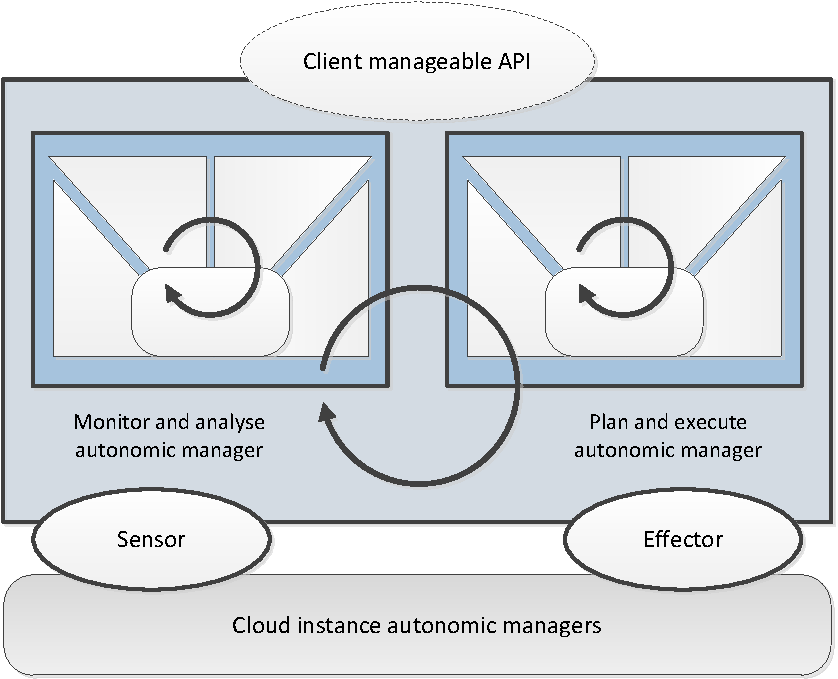
\includegraphics[width=0.7\textwidth]{chapter-design/csap-orchestrating-autonomic-manager}
  \end{center}
  \caption{Design of an orchestrating autonomic manager}
  \label{img:orchestrating-autonomic-manager}
\end{figure}

\subsection{Managed resource}
As it was stated in the previous sections and can be seen in figure \ref{img:orchestrating-autonomic-manager}, \emph{cloud instance autonomic managers} are managed resources of this manager. Each cloud instance is a deployment environment for a service or a stack, i.e. it is possible to span the service across different clouds by deploying stacks which make up the given service to different providers. Of course it is legitimate to deploy the whole service to only one provider.
\subsubsection*{Touchpoints}
As the cloud federation manager has to gain information about the state of a given cloud instance and be able to order the deployment of a stack or a service, the cloud instance exposes its manageability interface and its two types:
\begin{asparaenum}
\item[\textbf{Sensors}] -- set of attributes which forms the state of a given cloud instance. Attributes should include inter alia overall resources usage, pricing, geographical location. The more thorough elaboration will be held in the section devoted to \emph{plan and execution manager}.
\item[\textbf{Effectors}] -- set of stack/service management operations, such as deploy, migrate or delete.
\end{asparaenum}

\subsection{Plan and Execution Autonomic Manager}
The main purpose of this component is to select, based on knowledge provided directly to this manager from \emph{monitor and analyze manager} or a user (i.e. the specification of a service), cloud providers for a given service and carry out the planned action. In the following sections a detailed description of each function is given.

\subsubsection{Plan}
The aim of this function is to give a detailed plan for the action to be performed. In the context of this dissertation the first output produced by this component, regarding the use cases of deploying a service and dynamically scaling it, is a \emph{service deployment plan}, which is a mapping between available resources (cloud instances in this case) and concrete stacks making up the service. The second, definitely less complex, is a queries scheme about the state of the already-deployed services which is based on user's requests. In this case the component only propagates the request to the execute function. As this is only a mediation, there will be no further elaboration on this aspect.

\begin{asparaenum}
  \item[\textbf{Problem description}]
The problem of resource management in cloud computing environments is hard and complex. This is because of several aspects. The first one is the characteristic of resources available in a cloud -- not only are they geographically distributed, but they can be under different administrative domains and can vary in accessibility. This places a heavy burden on cooperation possibilities across cloud providers, both in a technical and non-technical way as providers need to maintain the high level of trust in order to effectively  deliver its products. Additionally, different entities forms the resources -- starting from individual devices, through virtual machines and whole workstations, ending with clusters and data centers. The second one are the increasing Quality-of-Service requirements from the clients. They want resources they use to be reliable, flexible (able to scale according to workload), fault-tolerant, energy-efficient and, of course, cheap. It is clear that clients and cloud vendors have different objectives and supply-and-demand patterns.

There are two main approaches to tackle the problem of effective resource management and scheduling:
  \begin{itemize}
    \item \textbf{conventional style}, in which the mapping decision is determined by some \emph{cost function}. The downside of this method is the fact that in many cases the decision is a function of system-centric parameters \cite{buyya2002economic} and because of it the outcome may lead to better utilization of cloud resources, not necessarily the user's application. What is more, this model treats all resources as if their cost was the same and applications are considered equally important what not always is the case. 

      The positive side of this method is the fact that it involves only one entity that governs the scheduling and allocating the resources. What is more, it is up to the platform how many factors should be incorporated in such a function. Depending on the needs, a more sophisticated or simpler matching algorithm be applied, e.g. an algorithm that takes into account only available budget of a client.
      
      Legion \cite{chapin1999legion} can be an example of a solution which uses this method.
    \item \textbf{economics-paradigm based} \cite{buyya2001case}, in which the decision is not made statically by one entity, but is driven by the users' requirements. The model tries to adopt the real-world economic solution that involves markets and brokers on the computational ground. In this paradigm, clients (representing \emph{demand}) want to solve their problems at the lowest possible price while assuring required Quality-of-Service requirements and constraints, such as time frame. Resource providers (representing \emph{supply}) want to maximise the utilization of their resources while keeping their prices at the level that is attractive for other customers.
      
      Here are the most common economic models which can be applied to resource scheduling and management \cite{buyya2002economic}:
      \begin{itemize}
        \item the commodity market model;
        \item the posted price model;
        \item the bargaining model;
        \item the tendering/contract-net model;
        \item the auction model;
        \item the bid-based proportional resource sharing model;
        \item the community/coalition/bartering model;
        \item the monopoly and oligopoly
      \end{itemize}
  \end{itemize}

\item[\textbf{Function input}] Depending on the actual request, this function can have access to different knowledge that makes its input:

  \begin{asparaenum}
  \item[\textbf{Service deployment}] When the user wants to deploy a service on a cloud infrastructure, they have to prepare its detailed description containing technical (stacks) and Quality-of-Service requirements.
  \item[\textbf{Service scaling}] When an application needs to be scaled, there is available additional knowledge that this component should use of -- detailed information about service's performance up to that point, e.g. service resource utilization level (CPU, I/O), response time, its users profile including their geographical location and so on. This knowledge in a form of a prediction model should be passed to the component by the \emph{analyse} function.
  \end{asparaenum}

\item[\textbf{Function output}] As it was stated in the introductory section, this function produces \emph{service deployment plan}. In the same section we conducted a quick survey of the most common approaches to the resource allocation and mapping problem. The proposed architecture places no restrictions on the chosen approach, as both paradigms can be fitted into it. In the case of \emph{conventional approach}, this component should be equipped with a matching function that takes as an input service description (and the information of its so far execution in the case of an auto-scaling action), offers from cloud providers and make a final decision based on these arguments.
  In the other case, this component can be thought of a cloud exchange \cite{InterCloud10}, that brings together service producers and consumers. Autonomic cloud instance managers could be considered bid-makers and would compete with one another for the client. What is more, if the model is bid-based, the client can have implemented behaviour that would also allow them to participate in auctions. This could be done by introducing another component that would act in user's name.
\end{asparaenum}

\subsubsection{Execute}
This function takes either a query about the state of a service or a deployment plan of the given service and passes execution requests to the proper cloud instance autonomic managers.
\subsection{Monitor and Analyse Autonomic Manager}

\section{Summary}
%podsumowanie, wyzwania stojace przed projektem, problemy ale takze obietnica dobrobytu i spokojnej starosci
